\documentclass[a4paper,12pt]{article}
% Package to change margin size
\usepackage{anysize}
\marginsize{2cm}{2cm}{1cm}{2cm}
% Package to make headers
\usepackage{fancyhdr}
\renewcommand{\headrulewidth}{0pt}
% Package for highligths
\usepackage{soul}

\usepackage[inline]{enumitem}

\usepackage{graphicx}
\usepackage{caption}
\newenvironment{Figure}
  {\par\medskip\noindent\minipage{\linewidth}}
  {\endminipage\par\medskip}

% Colors for the references links
\usepackage[dvipsnames]{xcolor}
% Package to link references
\usepackage{hyperref}
\hypersetup{
    colorlinks=true,
    linkcolor=black,
    citecolor=CadetBlue,
    filecolor=CadetBlue,      
    urlcolor=CadetBlue,
}
% Package for lorem ipsum
\usepackage{lipsum}
% Package for multicolumn
\usepackage{multicol}
% Package for removing paragraph identations
\usepackage{parskip}
\setlength\columnsep{18pt}
% Sets bastract
\renewenvironment{abstract}
 {\par\noindent\textbf{\abstractname}\ \ignorespaces \\}
 {\par\noindent\medskip}

 % Language
\usepackage[italian]{babel}

% Bibliography
\usepackage{csquotes}
\usepackage[
    backend=biber,
    style=alphabetic,
    sorting=ynt
]{biblatex}
\addbibresource{bib/bibliography.bib}



 
\begin{document}
% Makes header
\pagestyle{fancy}
\thispagestyle{empty}
\fancyhead[R]{\textit{F1801Q160: Machine Learning}}
\fancyhead[L]{}
% Makes footnotes with an asterisk
\renewcommand*{\thefootnote}{\fnsymbol{footnote}}
\begin{center}
\normalsize
Progetto finale per il corso F1801Q160: Machine Learning \\
\vspace{0.4cm}
\Large{\textbf{Riconoscimento di varietà di fagioli}}
\vspace{0.4cm}
\normalsize
\\ Mattia Bolognini, 870401 \\
\vspace{0.1cm}
\textit{Appello del 14 gennaio 2024}
\medskip
\normalsize
\end{center}
{\color{gray}\hrule}
\vspace{0.4cm}
\begin{abstract}
    Il progetto sviluppato prevede l'addestramento di più modelli di Machine
    Learning, il cui compito sarà quello di classificare un fagiolo nella 
    varietà a cui esso appartiene, in base alle sue caratteristiche (già
    individuate attraverso un altro modello di Computer Vision e relativa
    feature extraction).
    In particolare verrà effettuata una prima analisi del dataset, con relativa
    PCA per ridurre la dimensionalità dello spazio delle feature, per poi
    procedere con l'effettivo addestramento di quattro modelli di 
    classificazione: un albero decisionale, una rete neurale 
    (più precisamente un Multi Layer Perceptron), una Support Vector Machine e
    un Gaussian Naive Bayes classifier.
    Infine si confronteranno i vari modelli con metriche adatte, in modo da
    individuare quello più adatto al compito di classificazione dei fagioli.
\end{abstract}
{\color{gray}\hrule}
\medskip

\begin{multicols}{2}
    \tableofcontents

    \section{Introduzione}
\subsection{Descrizione del dominio}
Il dominio in cui si sta operando è quello dei fagioli, in particolare quello
delle loro varietà: ogni varietà di fagiolo ha, infatti, specifiche
caratteristiche che la contraddistinguono e che possono essere usate per
identificarle.

Lo studio di questo dominio ha importanti applicazioni pratiche, in 
quanto i fagioli secchi sono uno dei legumi più coltivati al mondo e la loro
coltivazione è fortemente legata alle loro varietà. 
Il processo di classificazione è, però, molto spesso svolto a mano 
da personale addetto e richiede quindi un alto costo e molto tempo.
Un modello di Machine Learning permetterebbe
quindi sia di velocizzare la selezione dei fagioli che di ridurre i costi.

\begin{Figure}
    \centering
    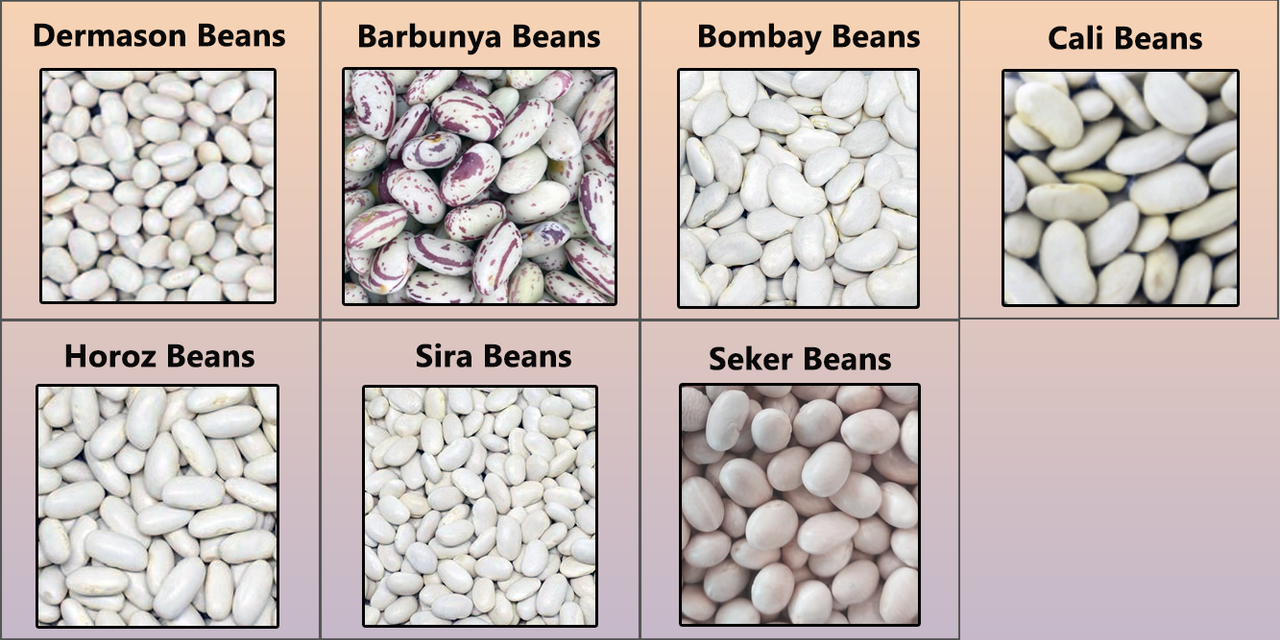
\includegraphics[width=\linewidth]{img/dry_beans.png}
    \captionof{figure}{Varietà di fagioli considerate.}
\end{Figure}

Il dominio analizzato si concentra su sole sette varietà di fagioli, in quanto
quelle più conosciute e interessanti agli autori originali del dataset:
Seker, Barbunya, Bombay, Cali, Dermosan, Horoz e Sira.

\subsection{Creazione del dataset}
Il dataset \cite{dry_bean_dataset} qui considerato è stato creato sfruttando un
sistema di computer vision, appositamente sviluppato dagli autori originali
per questo dominio: ogni fagiolo è stato, quindi, inquadrato singolarmente e ne 
è stata così ottenuta un'immagine in alta definizione.
A partire da ogni immagine, poi, il sistema ha effettuato segmentazione
e feature extraction: questo passaggio permette di evitare di trattare
i fagioli tramite i singoli pixel delle immagini che li rappresentano,
rendendoli analizzabili sfruttando molti meno dati molto più significativi,
come forma e dimensioni.
    \section{Analisi esplorativa}
\subsection{Descrizione del dataset}
Il dataset si compone di 13611 istanze, ognuna rappresentante un fagiolo
differente.
Sono presenti 16 feature, di cui 14 a valore continuo e 2 a valore intero.
4 di esse sono fattori di forma, mentre
le rimanenti 12 sono legate alla dimensione del fagiolo e alle
sue proporzioni.
Non sono presenti istanze con valori mancanti, e non è quindi necessario
adottare alcuna misura per gestire questo caso eccezionale.

Per quanto riguarda il target, invece, a ogni istanza è associata una label,
che corrisponde al nome della varietà a cui
essa appartiene. Per evitare di trattare label sottoforma di stringhe,
esse vengono tradotte, tramite label encoding, in interi maggiori o uguali a 0.
Il mapping che si ottiene è il seguente: Barbunya $\rightarrow$ 0, 
Bombay $\rightarrow$ 1, Cali $\rightarrow$ 2, Dermason $\rightarrow$ 3,
Horoz $\rightarrow$ 4, Seker $\rightarrow$ 5, Sira $\rightarrow$ 6.

Il dataset è fortemente sbilanciato, soprattutto le classi 3 e 5, che
presentano una differenza di 3000 istanze. 
\begin{Figure}
    \centering
    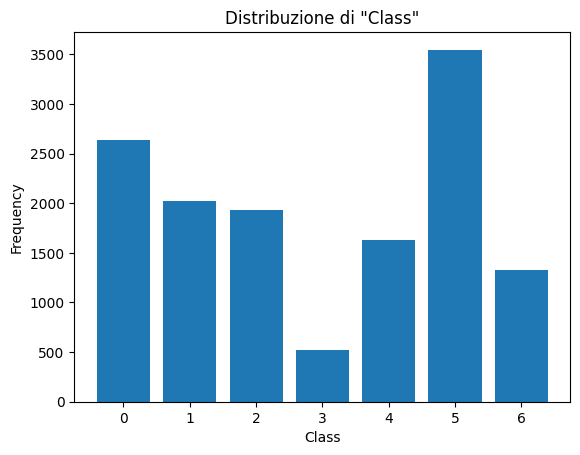
\includegraphics[width=\linewidth]{img/unbalanced_dataset.png}
    \captionof{figure}{Numero di istanze per classe.}
\end{Figure}
Per questo motivo non sarà possibile
utilizzare metriche di performance che non tengono conto di diversi costi
di errore per le classi, come l'accuratezza e la ROC-AUC, ma sarà necessario adottare misure
come la precisione, il richiamo, o l'f1-score (che corrisponde alla media
armonica tra precisione e richiamo).
Dovendo assegnare a tutte le classi la stessa importanza, inoltre, dovranno essere
preferite misure di macro-performance a quelle di micro-performance.

\subsection{Dimensionality reduction}
Ridurre la dimensionalità dello spazio delle istanze permette di ridurre la
complessità dei modelli e la probabilità di un loro eventuale overfitting.
La dimensionality reduction può essere effettuata rimuovendo feature superflue
e/o tramite PCA.

Il valore assunto da una feature dovrebbe idealmente dipendere solo
da fattori legati al dominio in cui si sta operando, e non al modo con cui 
si interagisce con il dominio stesso. 
In questo caso, però, 4 feature non dipendono esclusivamente dalla varietà a cui
il fagiolo appartiene, ma anche dalla distanza a cui esso è stato
inquadrato nella prima fase di Computer Vision. Queste 4 feature sono: 
Area, ovvero il numero di pixel occupati dal fagiolo; ConvexArea, ovvero il
numero di pixel occupati dalla più piccola figura convessa che racchiude
il fagiolo; MajorAxisLength, ovvero la lunghezza dell'asse maggiore dell'ellisse
con cui il fagiolo viene approssimato; MinorAxisLength, ovvero la lunghezza
dell'asse minore dell'ellisse che approssima il fagiolo.
Rimuovere semplicemente queste feature porterebbe, però, a un'importante perdita
di informazioni. Si può notare che i rapporti tra ConvexArea e Area
e tra MajorAxisLength e MinorAxisLength rimangono costanti al variare della
distanza di inquadratura, e possono essere utilizzati per caratterizzare una
varietà.
Ma questi rapporti sono già espressi da altre due feature del dataset,
rispettivamente Extent e AspectRatio, e quindi tutte e quattro le feature
citate possono essere rimosse, senza alcuna perdita di informazioni.

Una conseguenza molto importante della rimozione di queste feature è che le
due feature intere, Area e ConvexArea, non sono più presenti, rimanendo quindi con sole
feature continue: questo permetterà di applicare lo scaling e PCA a tutte le
feature e di usare il Gaussian Naive Bayes classifier senza preoccuparsi di
gestire le feature intere.

L'altra tecnica di dimensionality reduction che è possibile applicare è
la Principal Component Analysis, utile quando le feature sono fortemente correlate.
Prima ancora di effettuare la PCA, però, è necessario suddividere il dataset
in istanze di addestramento e istanze di test. La PCA verrà applicata, o per meglio
dire i coefficienti verranno calcolati, sulle sole istanze dedicate 
al training, mantenendo così una totale indipendenza tra istanze di addestramento
e istanze di test.
Essendo il dataset composto da una quantità medio-alta di istanze,
esso può essere suddiviso in
modo tale che le istanze di test coprano una percentuale tra il 20\% e 
il 40\% dell'intero dataset.
In questo caso, si è scelto di riservare il 25\% di istanze per il testing,
ottenendo, di conseguenza, 10208 istanze di addestramento e 3403 istanze di test.

Una volta effettuato lo splitting del dataset, è quindi possibile applicare la PCA.
Prima di farlo è però necessario effettuare lo scaling di tutte
le feature: la PCA, infatti, sceglie le componenti principali in base alla
loro varianza e feature con un'ampia scala, solitamente dotate di una 
varianza maggiore, potrebbero influenzare maggiormente la varianza delle
componenti principali e portare a una scelta artificiosa.
Lo scaling di una feature prevede di modificare tutti i suoi valori in modo 
che la sua media sia 0 e la sua varianza sia 1.

Il 95\% della varianza di questo dataset può essere espresso usando solo
5 componenti principali: il numero di feature si è quindi ridotto da 12 a 5.

\begin{Figure}
    \centering
    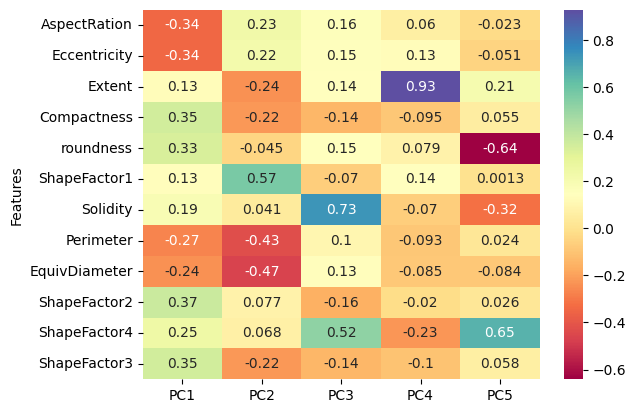
\includegraphics[width=\linewidth]{img/pca_features_weights.png}
    \captionof{figure}{Pesi delle feature per ogni componente principale.}
\end{Figure}

D'ora in poi, quando si parlerà di istanze di addestramento si farà riferimento
alle istanze di addestramento a cui è già stata applicata la PCA.
Si ricorda anche che, prima di poter utilizzare le istanze di test per verificare
le performance del modello, è necessario trasformarle usando lo stesso
scaler e le stesse componenti principali calcolati sulle istanze di addestramento. 

    \section{Addestramento}
Prima di procedere con l'addestramento, è necessario suddividere il dataset in
istanze di addestramento e istanze di test, che verranno poi utilizzate per verificare
le performance del modello addestrato. D'ora in poi, inoltre, non si farà più
riferimento al dataset originale, ma al dataset ottenuto dopo aver
applicato scaling e PCA.

Essendo il dataset composto da una quantità medio-alta di istanze,
esso può essere suddiviso in
modo tale che le istanze di test coprano una percentuale tra il 20\% e 
il 40\% dell'intero dataset.
In questo caso, si è scelto di riservare il 25\% di istanze al testing,
ottenendo, di conseguenza, 10208 istanze di addestramento e 3403 istanze di test.

Sono stati scegli 4 modelli di Machine Learning per affrontare il problema:
albero decisionale, Multi Layer Perceptron, Support Vector Machine e
Gaussian Naive Bayes classifier.
I primi tre modelli sono stati scelti in quanto, in base all'esperienza
maturata nell'intera
industria, essi si rivelano spesso performanti su feature estratte da immagini,
come avviene in questo caso.
Il quarto modello, ovvero Gaussian Naive Bayes, è stato invece scelto per provare
un approccio probabilistico al problema, e studiarne le performance. Inoltre,
anche Gaussian Naive Bayes si rivela essere molto spesso un buon classificatore
per feature estratte da immagini.

\subsection{Albero decisionale}
Un albero decisionale è un modello di Machine Learning che cerca di 
costruire un albero di classificazione. Ogni nodo interno corrisponde alla scelta
di una feature e al partizionamento dello spazio delle istanze associato in un 
numero di sottoinsiemi pari al numero di valori da essa assunti se la feature
è discreta, due se la feature è continua.
In questo ultimo caso, il primo sottoinsieme contiene le istanze il cui valore 
assunto dalla feature scelta è minore della sua media, mentre il secondo contiene
tutte le altre.
Le foglie rappresentano, invece, i nodi in cui viene effettivamente
effettuata la classificazione, in quanto a ognuna di esse è associata una classe.
Si può notare che, quando si trattano feature continue, la stessa feature può
essere usata più volte in uno stesso cammino radice-foglia.

La selezione di una feature per un certo nodo interno avviene in modo tale che 
essa sia quella che massimizza il miglioramento di una certa metrica 
se calcolata sul partizionamento definito dai suoi nodi figli. 
Esistono due metriche per la valutazione delle feature: indice di Gini ed entropia
di Shannon.

Per stabilire quale criterio permette di definire l'albero decisionale
migliore per il dataset che si sta considerando, si effettua una grid search
su entrambi i criteri, e si considera il modello con una maggiore
accuratezza bilanciata.
Per contenere la complessità dell'albero (e quindi l'overfitting), inoltre,
vengono valutati anche i parametri associati alla profondità massima
e al numero di foglie massimo.
I criteri di separazione che vengono valutati sono: \begin{itemize*}
    \item indice di Gini
    \item entropia di Shannon
\end{itemize*}.
I valori di profondità massima valutati sono: \begin{itemize*}
    \item 6
    \item 8
    \item 10
\end{itemize*}.
Il numero massimo di foglie può invece assumere i valori: \begin{itemize*}
    \item 20
    \item 25
    \item 35
\end{itemize*}.

\begin{Figure}
    \centering
    \includegraphics[width=\linewidth]{img/tree_plot.png}
    \captionof{figure}{Miglior albero decisionale.}
\end{Figure}

A seguito della grid search, il modello migliore si rivela essere quello la cui
combinazione di parametri è criterio = Gini, profondità massima = 8 e numero massimo
di foglie = 35.

Le performance del modello si rivelano essere ottime: si riscontrano un'accuratezza
bilanciata del $91\%$, una macro-precisione 
del $91\%$, un macro-recall del $91\%$ e un macro-f1 del $91\%$.

\begin{Figure}
    \centering
    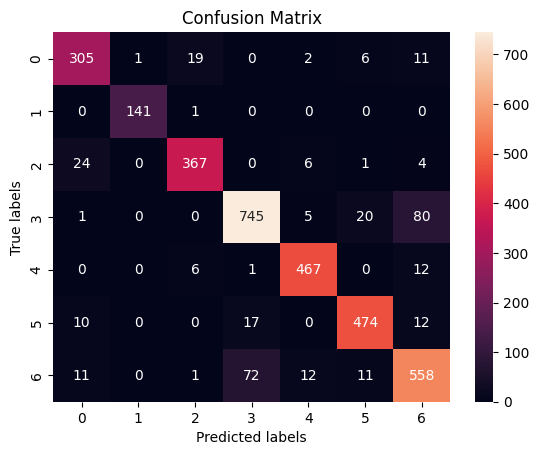
\includegraphics[width=\linewidth]{img/tree_confusion_matrix.png}
    \captionof{figure}{Matrice di confusione dell'albero decisionale.}
\end{Figure}

Si può notare una leggera confusione tra classe 3 e classe 6: 90 istanze che 
dovrebbero essere classificare come classe 3 vengono classificate come classe 6,
viceversa 50 istanze della classe 6 vengono classificate come classe 3.
Precisione e recall di entrambe le classi rimmangono comunque sopra all'$80\%$.

\subsection{Multi Layer Perceptron}
Un Multi Layer Perceptron è una rete neurale fully connected in cui 
ogni neurone si comporta come un percettrone. Una rete neurale è composta
da diversi strati di neuroni, che possono essere suddivisi in: strato di input;
strati nascosti; strato di output.
Un percettrone di uno strato nascosto attiva la sua connessione in output
sse il suo input pesato supera una certa soglia, detta soglia di attivazione.
L'apprendimento della rete avviene tramite la modifica dei pesi definiti
sulle connessioni tra neuroni: durante l'addestramento, la rete neurale esegue,
a intervalli regolari definiti dalla batch size, la backpropagation, ovvero
aggiorna i suoi pesi in modo tale da ridurre, idealmente, l'errore di previsione.
Per propagare l'errore, e quindi aggiornare i pesi, la rete usa la discesa del
gradiente, basata sulle derivate prime della funzione errore. Inoltre,
la discesa del gradiente necessita che le funzioni di attivazione dei neuroni
siano derivabili.
Le funzioni di attivazione derivabili più utilizzate sono lineare, tanh, relu
e softmax (solitamente usata per il layer di output). Alcune di esse, come tanh,
sono più computazionalmente onerose delle altre, come relu.
Ogni rete neurale, inotre, esamina l'input per un certo numero di epoche:
una singola analisi dell'intero dataset di addestramento corrisponde a un'epoca.

La complessità, e di conseguenza l'overfitting, di una rete neurale crescere
all'aumentare del numero di layer e del numero di neuroni contenuti in un
singolo layer: la rete deve quindi
essere definita in modo da ottenere alte performance con un numero limitato
di layer e neuroni per layer.
Un altro fattore di overfitting può essere l'esecuzione di molte epoche.

Per trovare la combinazione di parametri migliore per la rete, viene eseguita 
una grid search. 
I valori considerati per numero di layer layer e numero di nodi per layer sono:
\begin{itemize*}
    \item $(5, 5)$
    \item $(10)$
\end{itemize*}.
Le funzioni di attivazione considerate sono invece: \begin{itemize*}
    \item tanh
    \item relu
\end{itemize*}.

A seguito della grid search, la combinazione di parametri migliore si rivela essere 
layer = $(10)$ e funzione di attivazione = relu.

\begin{Figure}
    \centering
    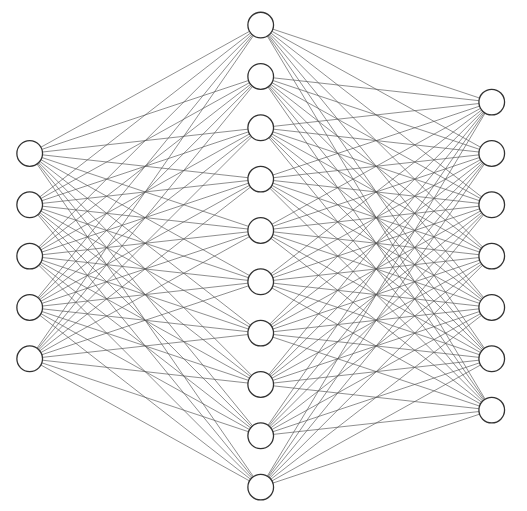
\includegraphics[width=0.75\linewidth]{img/mlp.png}
    \captionof{figure}{Multi Layer Perceptron con i parametri migliori.}
\end{Figure}

Le performance sono ottime: si rivela un'accuratezza bilanciata del $93,6\%$, una macro-precisione 
del $94\%$, un macro-recall del $94\%$ e un macro-f1 del $94\%$.

\begin{Figure}
    \centering
    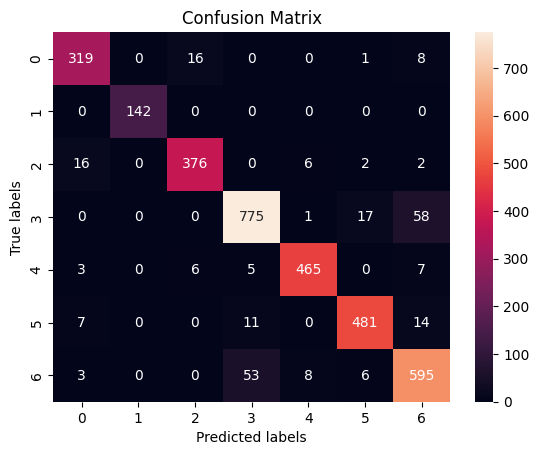
\includegraphics[width=\linewidth]{img/mlp_low_confusion_matrix.png}
    \captionof{figure}{Matrice di confusione del MLP.}
\end{Figure}

La complessità della rete rimane comunque elevata: analizzando la loss curve
definita nel corso dell'addestramento, infatti, si può evidenziare il fatto
che la loss non decresce significativamente per un elevato numero di epoche,
aumentando l'overfitting della rete sui dati di training e richiedendo un maggiore
tempo di addestramento. L'addestramento termina quindi al limite stabilito
dalla libreria Sklearn, ovvero 200 epoche.

\begin{Figure}
    \centering
    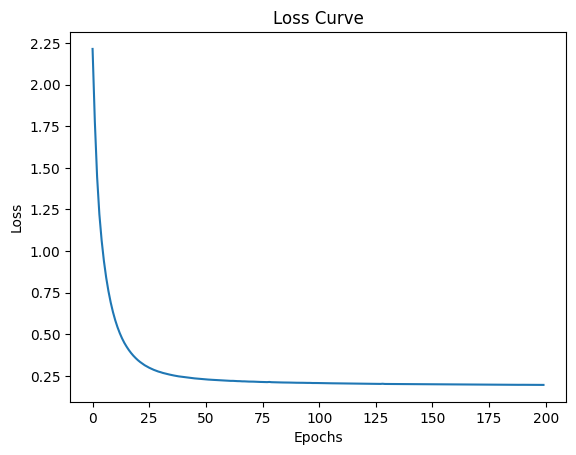
\includegraphics[width=0.9\linewidth]{img/mlp_low_loss.png}
    \captionof{figure}{Loss curve del MLP.}
\end{Figure}

Una tecnica che può essere utilizzata per ridurre il numero di epoche
è quella di aumentare la tolleranza della rete.
La tolleranza è, infatti, un parametro che stabilisce un decremento minimo
della loss durante l'esecuzione del training: se per 5 epoche la loss
diminuisce di un valore minore della tolleranza, allora il training si può
arrestare.
La tolleranza individuata che permette di mantenere performance simili alla
precedente rete è tol = 0.001. Rieffettuando il training, si può osservare che 
il numero di epoche si riduce a circa 80, dimezzando di fatto il numero
di epoche richieste.

\begin{Figure}
    \centering
    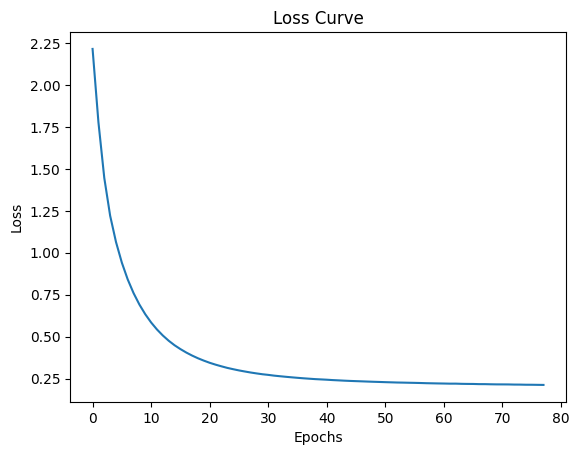
\includegraphics[width=0.9\linewidth]{img/mlp_high_loss.png}
    \captionof{figure}{Loss curve del MLP con tol = 0.001.}
\end{Figure}

Le performance della rete con una maggiore tolleranza sono anch'esse ottime:
si rileva un'accuratezza bilanciata del $93,4\%$, una macro-precisione 
del $94\%$, un macro-recall del $93\%$ e un macro-f1 del $93\%$.

\begin{Figure}
    \centering
    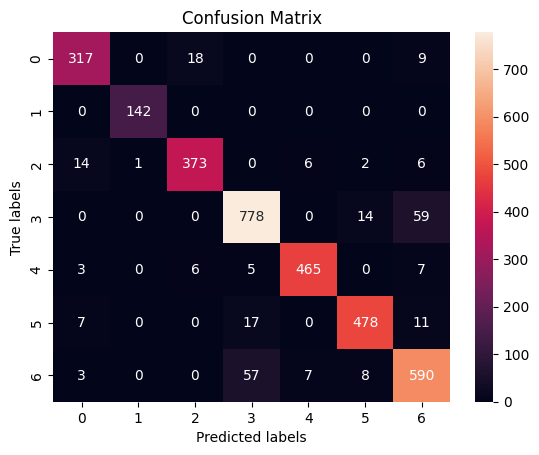
\includegraphics[width=\linewidth]{img/mlp_high_confusion_matrix.png}
    \captionof{figure}{Matrice di confusione del MLP con tol = 0.001.}
\end{Figure}

\subsection{Support Vector Machine}
Una Support Vector Machine è un modello di Machine Learning fortemente legato
al concetto di separabilità delle istanze: durante il suo addestramento, infatti,
essa cerca di separarle utilizzando degli iperpiani, in modo che istanze
appartenenti alla stessa classe ricadano nella stessa regione di spazio. 
Il numero di iperpiani di separazione necessari per classificare $n$ classi
è pari a $n-1$: in questo caso, quindi, saranno necessari 6 iperpiani, in quanto
le varietà di fagioli considerate sono 7.

L'apprendimento di una SVM "pura" converge, però, sse le istanze
sono linearmente separabili.
Esistono quindi due tecniche che permettono di trattare anche dataset non linearmente
separabili: soft-margin e kernel trick.

La prima tecnica, il soft-margin, consiste nel tollerare una certa quantità di
errore, e permettere quindi una misclassificazione di un numero ridotto di
istanze. La quantità di errore tollerata viene determinata da un parametro $C$,
detto trade-off, che deve essere stabilito prima dell'apprendimento.
Al crescere di $C$, l'errore tollerato si riduce e la complessità del modello
aumenta.

Il kernel trick permette, invece, di separare le istanze utilizzando funzioni non
lineari. In realtà, il kernel trick non separa le istanze con vere e proprie
funzioni non lineari, ma le separa linearmente in uno spazio di dimensione
maggiore di quello di partenza; questo 
iperpiano, però, si traduce in una funzione non lineare nello spazio di partenza.
Anche in questo caso, il kernel che deve essere utilizzato per aumentare la
dimensionalità dello spazio deve essere stabilito prima dell'apprendimento.
Le funzioni kernel più comuni sono: \begin{itemize*}
    \item lineare
    \item polinomiale
    \item radial basis function (rbf).
\end{itemize*}

Prima di procedere con l'addestramento, è necessario anche effettuare un'osservazione
sulle scale delle feature: una SVM è, infatti, sensibile a feature con diverse scale,
e risulta più performante su dataset a cui è stato applicato lo scaling.
Questo passaggio è, però, già stato effettuato nella fase di Analisi esplorativa.

Viene quindi eseguita una grid search per individuare la combinazione di parametri
migliore, ovvero quella che massimizza l'accuratezza bilanciata.
I valori di trade-off considerati sono: \begin{itemize*}
    \item 1
    \item 2
    \item 5
\end{itemize*}.
I kernel considerati sono invece: \begin{itemize*}
    \item lineare
    \item polinomiale
    \item radial basis function (rbf)
\end{itemize*}.

A seguito della grid search, la combinazione migliore si rivela essere $C=2$ e
kernel = rbf. Di conseguenza, la complessità del modello è abbstanza contenuta,
grazie al basso valore di $C$.
Il numero di vettori di supporto individuati da questa SVM è pari a 2151.

Le perfomance della SVM addestrata con questi parametri sono ottime:
viene rilevata un'accuratezza bilanciata del $94,2\%$, una macro-precisione 
del $94\%$, un macro-recall del $94\%$ e un macro-f1 del $94\%$.

\begin{Figure}
    \centering
    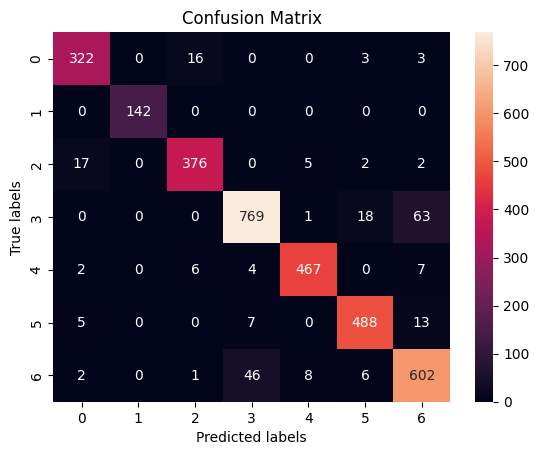
\includegraphics[width=\linewidth]{img/svm_confusion_matrix.png}
    \captionof{figure}{Matrice di confusione della SVM.}
\end{Figure}

\subsection{Gaussian Naive Bayes}
Gaussian Naive Bayes classifier è un modello di Machine Learning basato sul
teorema di Bayes: a ogni nuova istanza di addestramento analizzata, infatti,
il modello aggiorna le probabilità delle classi usando proprio il teorema di Bayes.
La classificazione avviene, invece, scegliendo la classe di probabilità maggiore
data l'istanza che si vuole classificare.
Gaussian Naive Bayes è la variante del Naive Bayes classifier che può essere applicata
a dataset con feature continue (Naive Bayes può infatti trattare solo feature 
discrete) e con valori negativi.

Questo classificatore si può utilizzare solo facendo alcune
assunzioni: la distribuzione di probabilità di ogni feature deve essere
normale e ogni feature deve essere condizionalmente indipendente dalle altre.
Per quanto riguarda la seconda assunzione, le componenti principali del dataset
hanno tutte distribuzioni normali, escluse la prima e la seconda. 
Si possono comunque assumere normali, in modo da poter ugualmente applicare il 
classificatore gaussiano.
Inoltre, tutte le feature con varianza 0 non devono essere considerate, in quanto
non portano alcuna informazione e non permettono al classificatore di 
raggiungere performance ottimali. Si può osservare, però, che le uniche feature
rimaste sono le 5 componenti principali scelte da PCA, ognuna con varianza
strettamente maggiore di 0.

\begin{Figure}
    \centering
    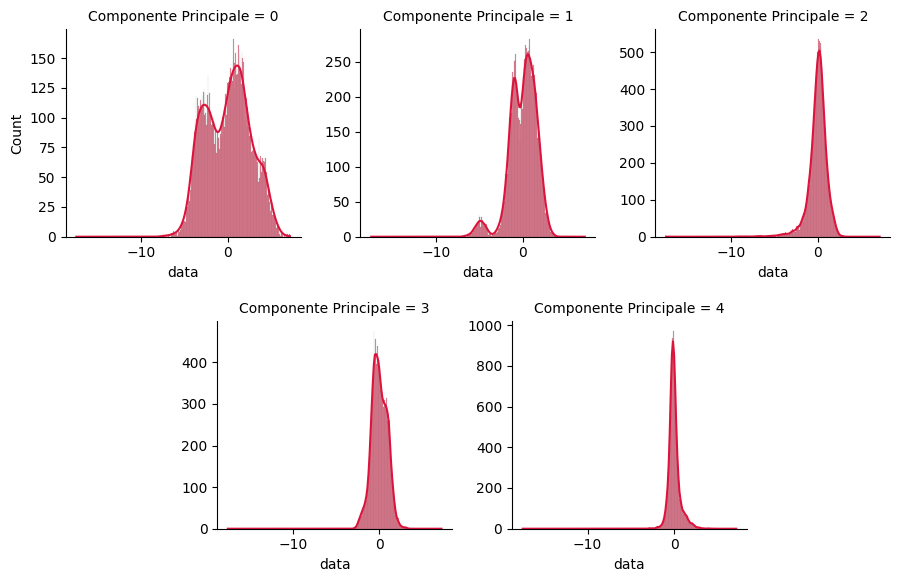
\includegraphics[width=0.85\linewidth]{img/components_distribution.png}
    \captionof{figure}{Distribuzioni di probabilità per le componenti principali
    considerate.}
\end{Figure}

\begin{Figure}
    \centering
    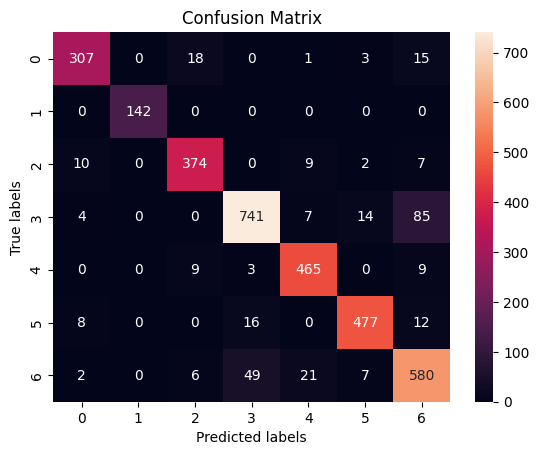
\includegraphics[width=\linewidth]{img/gnb_confusion_matrix.png}
    \captionof{figure}{Matrice di confusione di Gaussian Naive Bayes.}
\end{Figure}

Nonostante tutte queste assunzioni, il classificatore gaussiano si rivela essere
molto performante e velocissimo da addestrare: si riscontra un'accuratezza 
bilanciata del $92,2\%$, una macro-precisione 
del $92\%$, un macro-recall del $92\%$ e un macro-f1 del $92\%$.

    \section{Confronto tra modelli}
I quattro modelli addestrati portano tutti a ottime performance, ma i loro 
tempi di addestramento variano notevolmente.
Per scegliere il modello migliore, quindi, vengono analizzati sia il macro-f1 score
sia il tempo di addestramento.

Per calcolare valore medio e intervallo di confidenza di entrambe
le misurazioni, viene eseguita
una stratified cross-validation con 10 fold. Questo numero di fold è stato 
scelto perchè esperimenti passati hanno dimostrato che un tale numero di fold
permette di approssimare bene i valori reali.

Per quanto riguarda il macro-f1 score, tutti i modelli presentano un
valore medio maggiore del $90\%$. In particolare, i valori medi dei quattro modelli
sono: \begin{itemize*}
    \item albero decisionale = $91,1\%$
    \item MLP = $93,2\%$
    \item SVM = $93,8\%$
    \item Gaussian Naive Bayes = $91,5\%$
\end{itemize*}
Gli intervalli di confidenza al $90\%$ del macro-f1 score sono invece:
\begin{itemize*}
    \item albero decisionale = $(90,7\%, 91,4\%)$
    \item MLP = $(92,9\%, 93,5\%)$
    \item SVM = $(93,6\%, 94,1\%)$
    \item Gaussian Naive Bayes = $(91,1\%, 91,8\%)$
\end{itemize*}
Il modello con le performance migliori è, quindi, la SVM.

\begin{Figure}
    \centering
    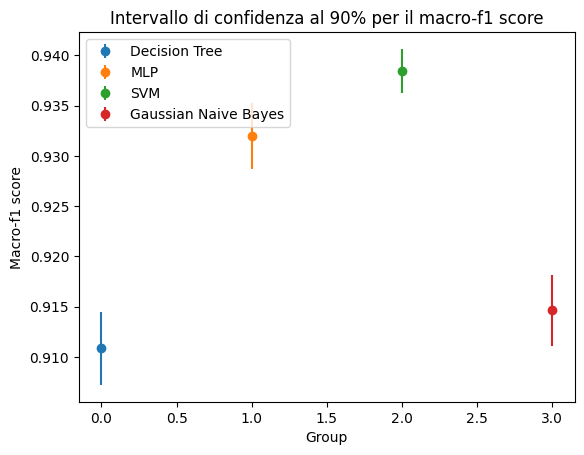
\includegraphics[width=\linewidth]{img/confidence_interval_perf.png}
    \captionof{figure}{Intervallo di confidenza al 90\% per il macro-f1 score.}
\end{Figure}

Analizzando i tempi di addestramento medi, però, si può osservare che
SVM e MLP richiedono molto più tempo per essere addestrate rispetto
agli altri due modelli: \begin{itemize*}
    \item albero decisionale = 88 ms
    \item MLP = 2003 ms
    \item SVM = 987 ms
    \item Gaussian Naive Bayes = 5 ms
\end{itemize*}
L'intervallo di confidenza al $90\%$ del tempo di addestramento è: \begin{itemize*}
    \item albero decisionale = (82 ms, 94 ms)
    \item MLP = (1617 ms, 2389 ms)
    \item SVM = (817 ms, 1156 ms)
    \item Gaussian Naive Bayes = (4 ms, 5 ms)
\end{itemize*}

\textit{NOTA}: i tempi di esecuzione qui riportati non possono essere identici a quelli 
rilevati su Colab. 
Il tempo di esecuzione dipende, infatti, da molti fattori, tra cui il 
carico dei server di Google Colab. Si può affermare, però, che i tempi qui
riportati approssimano bene il tempo di addestramento reale.

\begin{Figure}
    \centering
    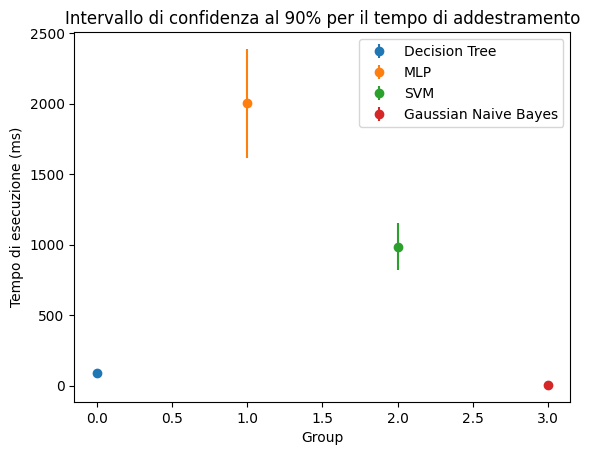
\includegraphics[width=\linewidth]{img/confidence_interval_time.png}
    \captionof{figure}{Intervallo di confidenza al 90\% per il tempo di addestramento.}
\end{Figure}

Tutti i modelli addestrati presentano, quindi, ottime performance.
La scelta del modello migliore, che verrà effettivamente usato 
per la classificazione dei fagioli, ricade principalmente, quindi,
sul tempo di addestramento.
La rete neurale, offrendo prestazioni poco inferiori alla SVM ma con un tempo 
di addestramento maggiore, è il primo modello che è possibile scartare.
Lo stesso ragionamento può essere applicato all'albero decisionale,
in riferimento al Gaussian Naive Bayes classifier.
Tra i due modelli rimanenti, ovvero SVM e Gaussian Naive Bayes, la scelta dipende
dalla tolleranza all'errore che il dominio sopporta: se, infatti,
le performance devono essere massimizzate, allora la scelta ricade sulla SVM, 
e dovranno essere tollerati tempi di addestramento maggiori.
Se, invece, il dominio di applicazione sopporta permormance minori (che in questo
caso sono comunque ottime, in quanto Gaussian Naive Bayes ha un
macro-f1 score medio del $91,5\%$), allora è possibile scegliere Gaussian Naive Bayes,
e beneficiare di tempi di addestramento molto ridotti.

Nel dominio di applicazione considerato in questo progetto, ovvero la classificazione
di fagioli nelle loro varietà, alcuni errori possono essere tollerati, 
in quanto campo a basso impatto d'errore. Di conseguenza, il modello che
sarà mandato in produzione sarà il Gaussian Naive Bayes.
    \section{Conclusioni}
Tutti i modelli scelti ottengono ottime performance sul dataset: si riscontrano
sempre, infatti, macro-precisione, macro-recall e macro-f1 score maggiori del 90\%.
Come già affermato, però, i tempi di addestramento variano notevolmente,
e la scelta del migliore modello deve essere dettata anche da questo fattore.
Dopo un'attenta analisi, si è deciso che il modello più adatto al dominio considerato
è il Gaussian Naive Bayes, con un macro-f1 score medio del $91,5\%$
e un tempo di addestramento quasi istantaneo, che si aggira intorno ai 6 ms. 

Questo modello permetterà di diminuire il tempo richiesto per la classificazione,
dei fagioli, e i costi saranno notevolmente ridotti, in quanto non sarà più 
necessario assumere personale addetto (o comunque lo si farà in maniera molto ridotta).
Il principale costo associato al sistema di riconoscimento automatico sarà
solo l'investimento iniziale per l'acquisto del sistema stesso.

    \printbibliography
\end{multicols}

\end{document}